The following formulas are of the most essential trigonometric formulas that 
will be utilized in the subsequent text, their proof is attached by the end of this section: 

\begin{itemize}
    \item \( \cos{(\phi \pm \alpha)} = \cos{(\phi) \cdot \cos{(\alpha)}} 
            \mp \sin{(\phi)} \cdot \sin{(\alpha)} \)    <<1>> 
    \item \( \sin{(\phi \pm \alpha)} = \sin{(\phi)} \cdot \cos{(\alpha)} 
            \pm \cos{(\phi)} \cdot \sin{(\alpha)} \)    <<2>> 
    \item \( \tan{(\phi \pm \alpha)} = \frac{\tan{\phi} \pm \tan{\alpha}}{1 \mp \tan{\phi} \cdot \tan{\alpha}} \)  <<3>>

\end{itemize}

\specialsubsection{Proof for equation (1) using Vector Maths from Calculus II:}{
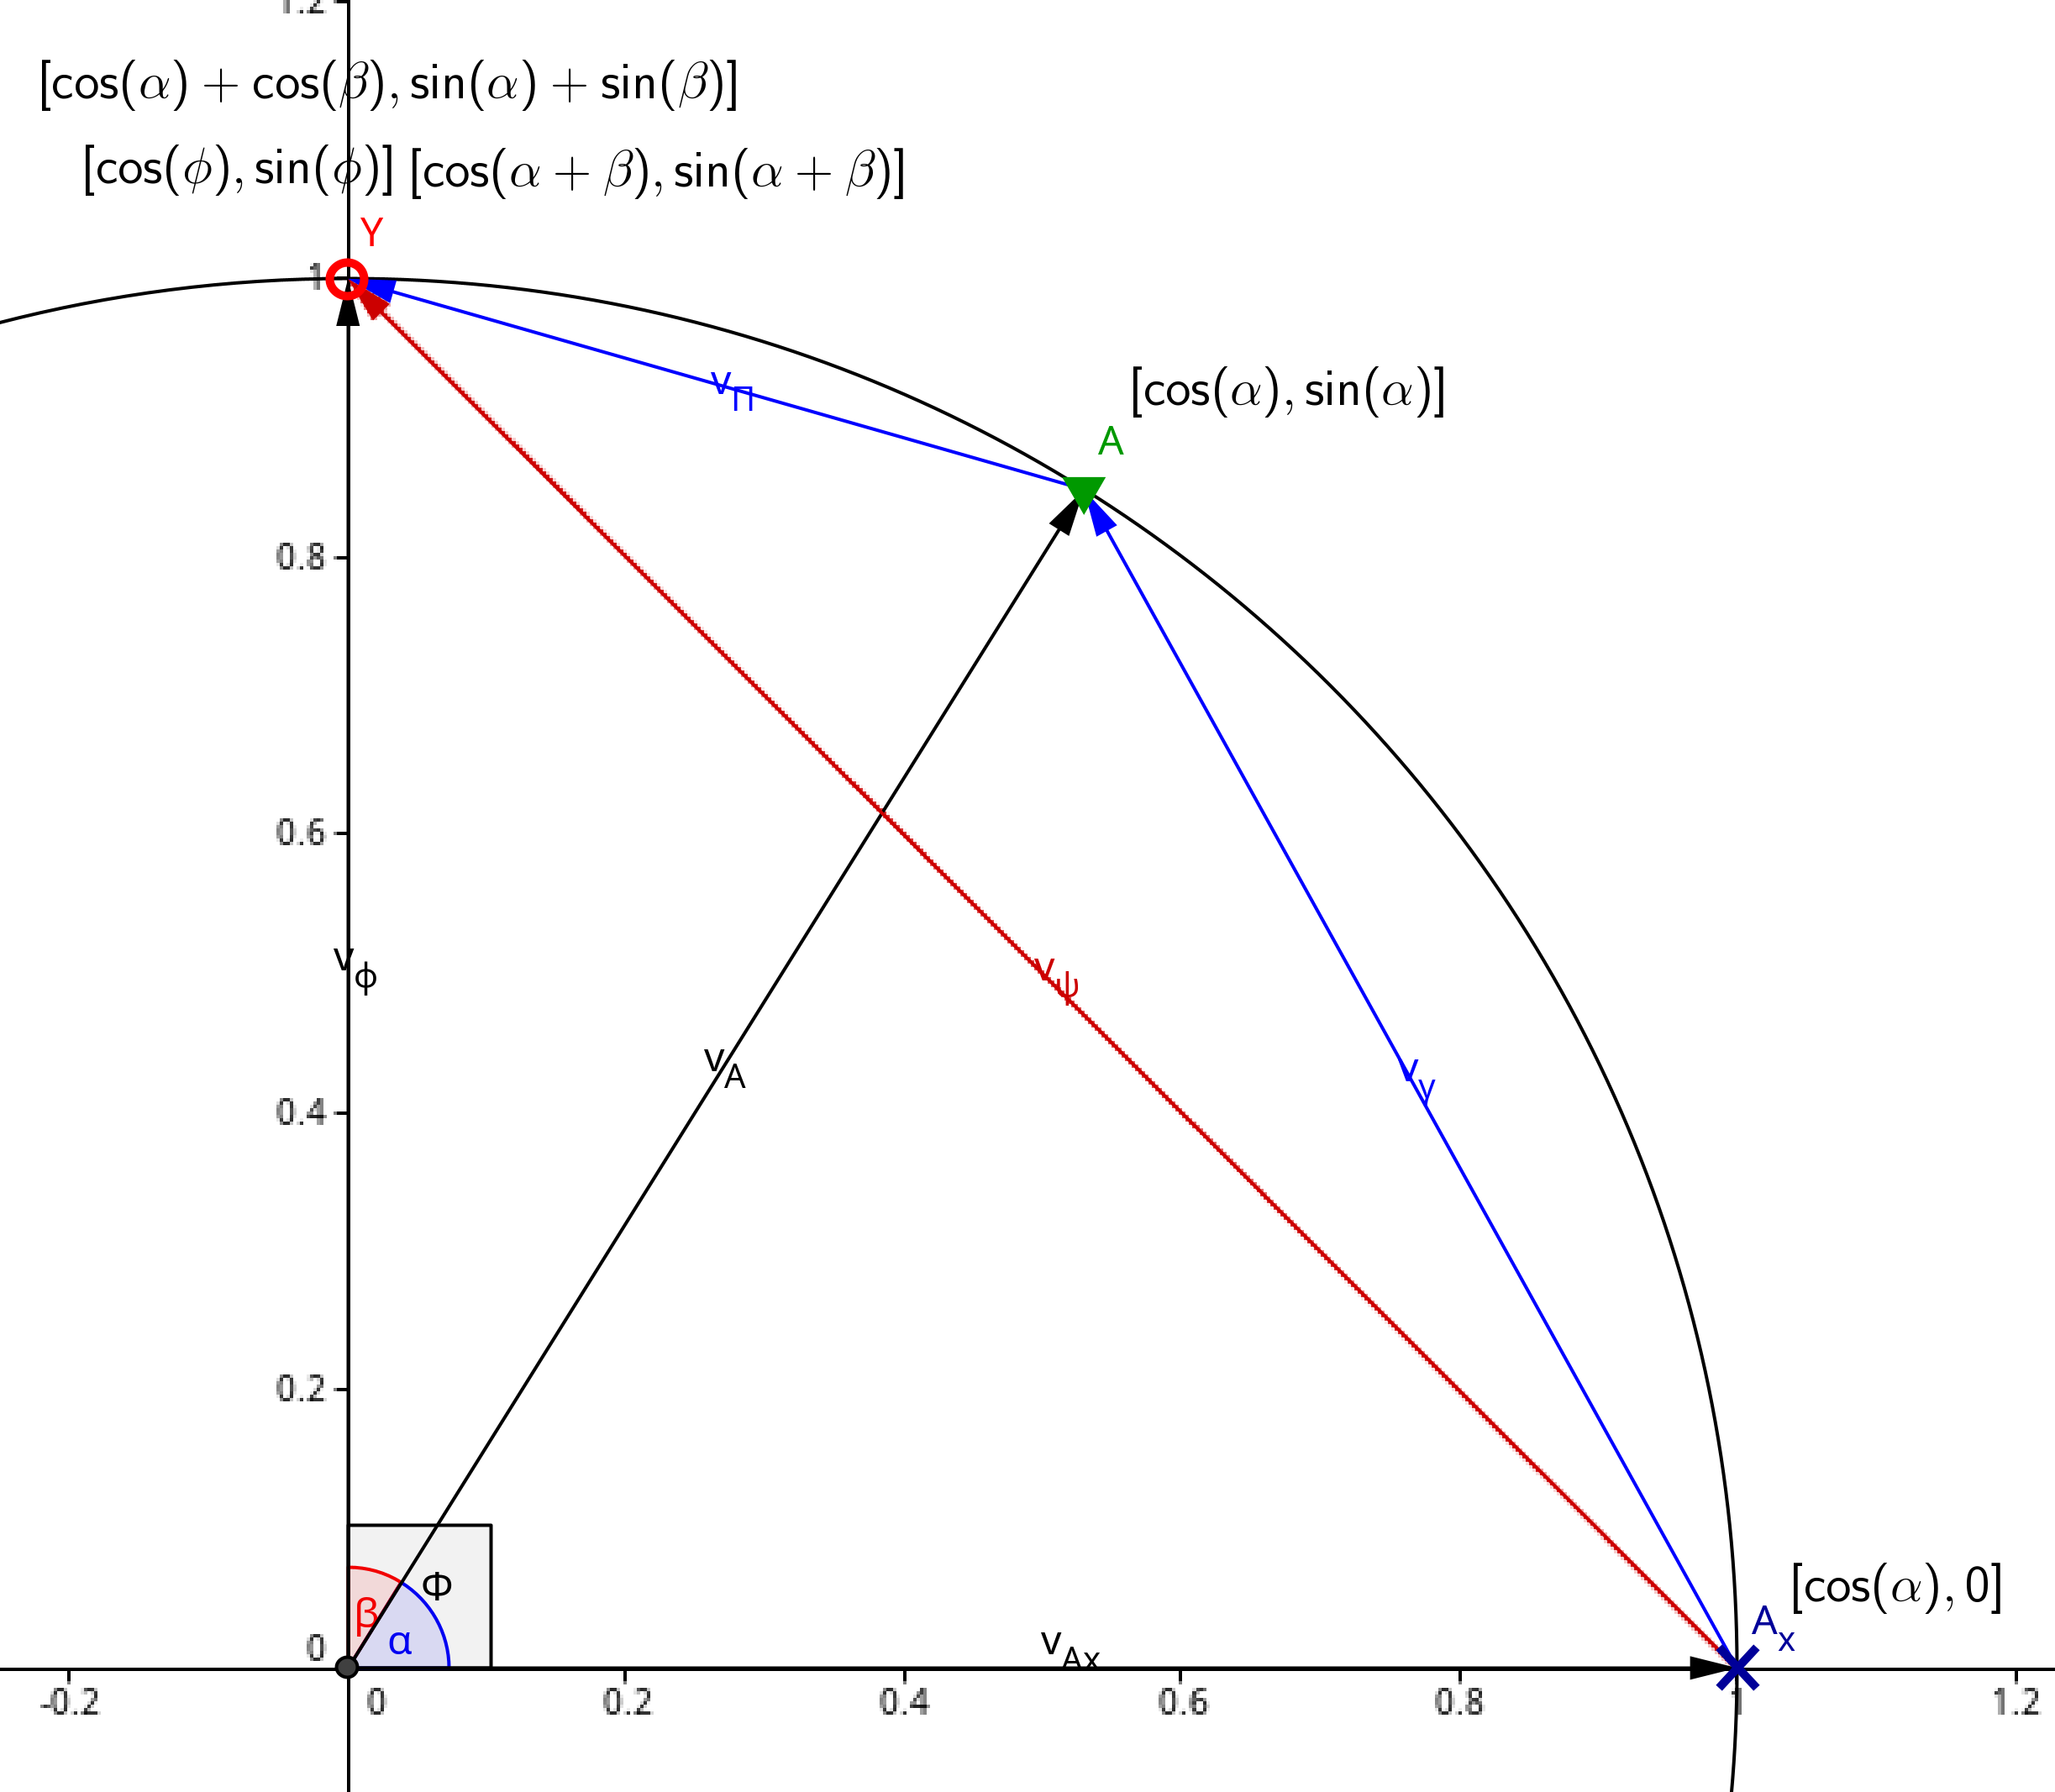
\includegraphics{proof-1.png} 
\\\\ 
\(   
\because
\vec{\Phi} = \vec{\Phi} - \vec{\rho} 
           = (\vec{{\Phi}_x} + \vec{{\Phi}_y}) - \vec{\rho}
            = (\begin{bmatrix}
            \cos{\phi} \\
            0
            \end{bmatrix} + \begin{bmatrix}
            0 \\
            \sin{\phi}
            \end{bmatrix}) - \begin{bmatrix}
            0 \\
            0
            \end{bmatrix} = \begin{bmatrix}
                            \cos{\phi} \\
                            \sin{\phi}
                            \end{bmatrix} \)

\( 
\vec{A} = \vec{A} - \vec{\rho}
             = (\vec{{A}_x} + \vec{{A}_y}) - \vec{\rho}
             = \begin{bmatrix}
                \cos{\alpha} \\
                \sin{\alpha}
                \end{bmatrix}
\)

\(
\vec{\psi} = \vec{\psi} - \vec{\rho}
           = (\vec{{\psi}_x} + \vec{{\psi}_y}) - \vec{{A}_x}
           = \vec{\upsilon} + \vec{\Pi}
\)

\(
\vec{\upsilon} = \vec{\upsilon} - \vec{\rho} 
               = \vec{A} - \vec{A_x}
               = \begin{bmatrix}
                0 \\
                \sin{\alpha}
                \end{bmatrix}
\)

\begin{equation}
\therefore \vec{\Pi} = \vec{\Pi} - \vec{\rho} 
          =  \begin{bmatrix}
            \cos{\beta} \\
            \sin{\beta}
            \end{bmatrix} - \vec{\rho}    
            \\
          = \vec{\Phi} - \vec{A} 
          =  \begin{bmatrix} 
            \cos{\phi} - \cos{\alpha} \\
            \sin{\phi} - \sin{\alpha}
            \end{bmatrix}
\end{equation}


Essentially, in order to compute for $\angle{\beta}$ in an $R^2$ vectorspace, the initial side angle 
must align with the \(+'ve\) direction of the x-axis. 
\\\\
\(\because \vec{\Pi}\) is translated by vector \(\vec{A}\)
of polar coordinates \([\cos{\alpha}, \sin{\alpha}]\) then to
align \(\vec{\Pi}\) to the \(+'ve\) direction of the x-axis, one extra
operation should be attained, a vector translation transformation that 
could be carried on through the preset vector \( \vec{\rho} \):
\\
\(
\vec{\Pi} = \vec{\Pi} - \vec{\rho} \\
          = (\vec{A} + \vec{\Pi}) - \vec{A} \\
          = \begin{bmatrix}
            (\cos{\alpha} + \cos{\beta}) - \cos{\alpha}\\
            (\sin{\alpha} + \sin{\beta}) - \sin{\alpha}
            \end{bmatrix} \\
          = \begin{bmatrix}
            \cos{\beta} \\
            \sin{\beta}
            \end{bmatrix} \\
\)
\\ 
After this transformation, vector \(\vec{\Pi}\) aligns perfectly with the 
\(+'ve\) direction of x-axis rendering computing angle \(\angle{\beta}\) straightforward,
and hence the vector \(\vec{\Pi}\) can be calculated using distance operations: 
\\ 
\(
\vec{\Pi} = \vec{\Pi} - \vec{\rho} \\
          = \vec{\Pi} - \vec{x} \\
          = \begin{bmatrix}
            \cos{\beta} - 1\\
            \sin{\beta} - 0
            \end{bmatrix} \\
\)
\\
\begin{equation}
\because 
\angle{\phi} = \angle{\alpha} + \angle{\beta} \\
\\
\therefore \angle{\beta} = \angle{\phi} - \angle{\alpha} \\
\\
\therefore \vec{\Pi} = \begin{bmatrix}
    \cos{(\phi - \alpha)} - 1\\
    \sin{(\phi - \alpha)}
    \end{bmatrix} \\
\end{equation}
\\
\( \therefore, from (1) and (2), \) we can deduce that the following norms are equal:
\\
\(
\sqrt{{(\cos{\phi} - \cos{\alpha})}^2 + {(\sin{\phi} - \sin{\alpha})}^2} \\
= \sqrt{{(\cos{\phi - \alpha} - 1)}^2 + {(\sin{\phi - \alpha})}^2} 
\\ \cdots \\
2 \cdot (1 - \cos{(\phi - \alpha)}) = 2 \cdot (1 - \cos{\phi}\cdot\cos{\alpha} - \sin{\phi}\cdot\sin{\alpha})
\\ \cdots \\
\)
\specialsubsection{The Cosine Addition Formula}{
\[
\therefore \cos{(\phi - \alpha)} = \cos{\phi}\cdot\cos{\alpha} + \sin{\phi}\cdot\sin{\alpha}
\]
}{red}

}{black}

\specialsubsection{Proof for equation (2) using the Co-Function forumlas}{
\( \because \sin{\theta} = \cos{(\frac{\pi}{2} - \theta)} \); as both cosine and sine functions are co-functions
in the same right-angled triangle or among 2 similar right-angled triangles in a unit circle.
\\\\
\(
\sin{(\phi \pm \alpha)} = \cos{(\frac{\pi}{2} - (\phi \pm \alpha))} 
                      = \cos{((\frac{\pi}{2} - \phi) \mp \alpha)} \\
                      = \cos{(\frac{\pi}{2} - \phi)}\cdot\cos{\alpha} \pm \sin{(\frac{\pi}{2} - \phi)}\cdot\sin{\alpha} \\
                      = \sin{\phi}\cdot\cos{\alpha} \pm \cos{\phi}\cdot\sin{\alpha}
\)
\specialsubsection{The Sine Addition Formula}{
\[
\therefore \sin{(\phi \pm \alpha)} = \sin{\phi}\cdot\cos{\alpha} \pm \cos{\phi}\cdot\sin{\alpha}
\]
}{red}
}{black}

\specialsubsection{Proof for equation (3) using the Tangent fundamental identities}{
\( \because \tan{\theta} = \frac{\sin{\theta}}{\cos{\theta}} \), and from (1) and (2):
\\
\begin{equation} 
\tan{(\phi \pm \alpha)} = \frac{\sin{(\phi \pm \alpha)}}{\cos{(\phi \pm \alpha)}} \\
             = \frac{
                \sin{\phi}\cdot\cos{\alpha} \pm \cos{\phi}\cdot\sin{\alpha}
             }{
                \cos{\phi}\cdot\cos{\alpha} \mp \sin{\phi}\cdot\sin{\alpha}
             }
\end{equation}
\\ 
\( \because \tan{\theta} = \frac{\sin{\theta}}{\cos{\theta}} \\
    \therefore \sin{\theta} = \cos{\theta}\cdot\tan{\theta} 
\)
\\
\(  
\therefore \tan{(\phi \pm \alpha)} =  \frac{
    \tan{\phi}\cdot\cancel{\cos{\phi}\cdot\cos{\alpha}} \pm \cancel{\cos{\phi}\cdot\cos{\alpha}}\cdot\tan{\alpha}
 }{
    \cancel{\cos{\phi}\cdot\cos{\alpha}} \mp \cancel{\cos{\phi}\cdot\cos{\alpha}}\cdot\tan{\alpha}\cdot\tan{\phi}
 }
\)
\\
\specialsubsection{The Tangent Addition Formula}{
\[
    \therefore \tan{(\phi \pm \alpha)} = \frac{
        \tan{\phi} \pm \tan{\alpha}
     }{
        1 \mp \tan{\alpha}\cdot\tan{\phi}
     }
\]
}{red}

}{black}

\specialsubsection{Extra Verification Proofs done differently}{
\specialsubsection{
Verify that: \(
\sin{(\phi + \frac{3\pi}{2})} = - \cos{\phi}
\)
\\
}{

\begin{proof}
\begin{equation} 
\because \sin{(\phi + \frac{3\pi}{2})} = \sin{(\phi + \pi + \frac{\pi}{2})}
                                       = \sin{(\frac{\pi}{2} - (-\phi - \pi))}
\end{equation}

\begin{equation} 
\because \sin{(\frac{\pi}{2} - \alpha)} = \cos{\alpha} 
\end{equation}

\begin{equation}
         \cos{(-\alpha)} = \cos{\alpha}
\end{equation} 


\( \therefore \) from (4), (5), \& (6):
\\
\(
\sin{(\phi + \frac{3\pi}{2})} = \sin{(\frac{\pi}{2} - (-\phi - \pi))} \\
                              = \cos{(-\phi - \pi)} \\
                              = \cos{(-(\phi + \pi))} \\
                              = \cos{(\phi + \pi)} \\
                              = - \cos(\phi)
\)
\end{proof}
}{red}
}{black}